\documentclass[UTF8,a4paper]{paper}
\usepackage{ctex}
\usepackage[utf8]{inputenc}
\usepackage{amsmath}
\usepackage{pdfpages}
\usepackage{graphicx}
\usepackage{wrapfig}
\usepackage{listings}
\usepackage{multicol}
\usepackage{float}
\newcommand{\tabincell}[2]{\begin{tabular}{@{}#1@{}}#2\end{tabular}}
\title{实验四\ \ 波形发生电路仿真及实验}
\author{张蔚桐\ 2015011493\ 自55}
\begin {document}
\maketitle
\section{仿真和预习}
\subsection{正弦波发生电路}
\subsubsection{理论计算}
\begin{multicols}{2}
\begin {figure}[H]
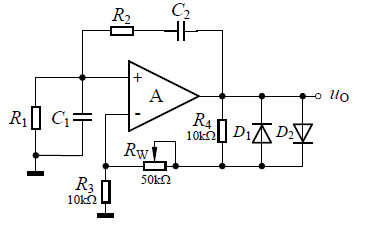
\includegraphics [width=\columnwidth]{ac.png}
\caption{正弦波发生电路}
\label{ACCirc}
\end {figure}
\end{multicols}
\subsubsection{输出波形调试}
\begin {figure}[H]
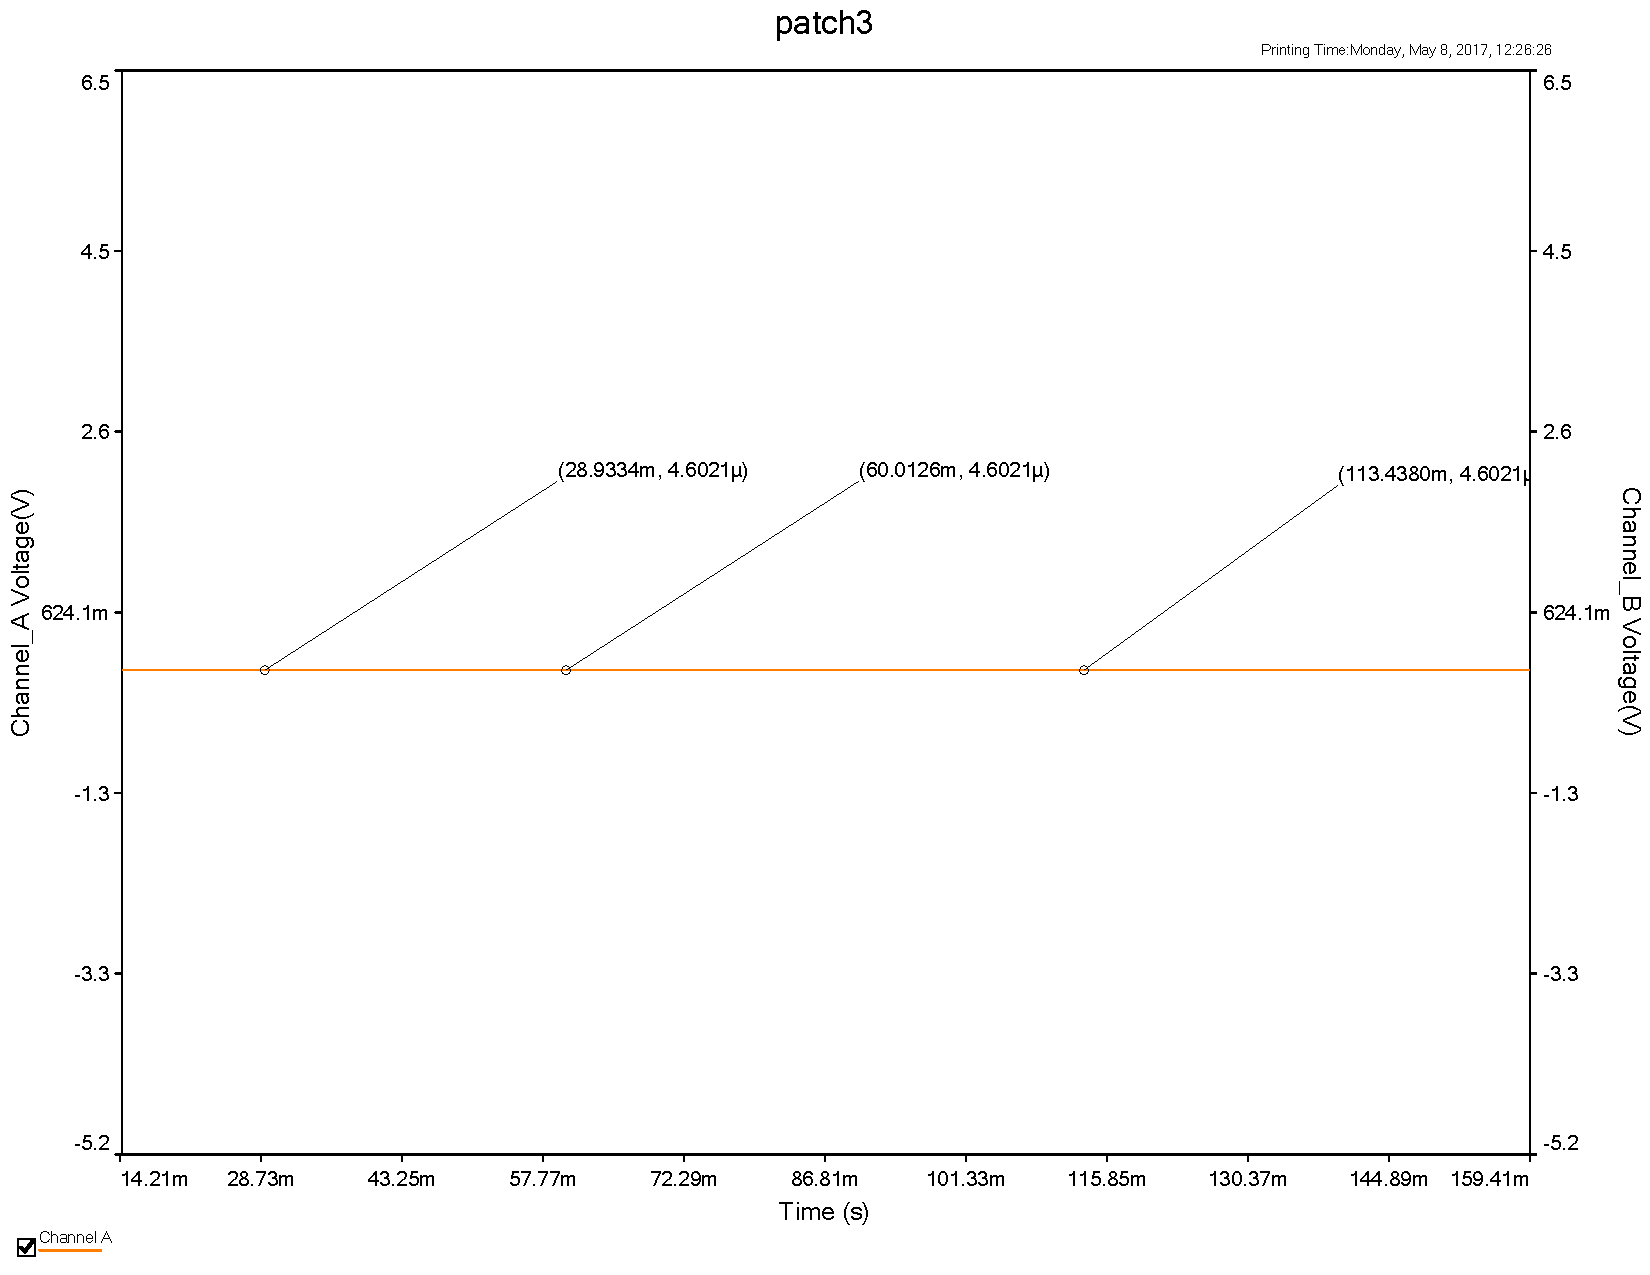
\includegraphics [width=\textwidth]{0ac.pdf}
\caption{$R_w=0$时的输出波形}
\label{AC0}
\end {figure}
\begin {figure}[H]
\centering
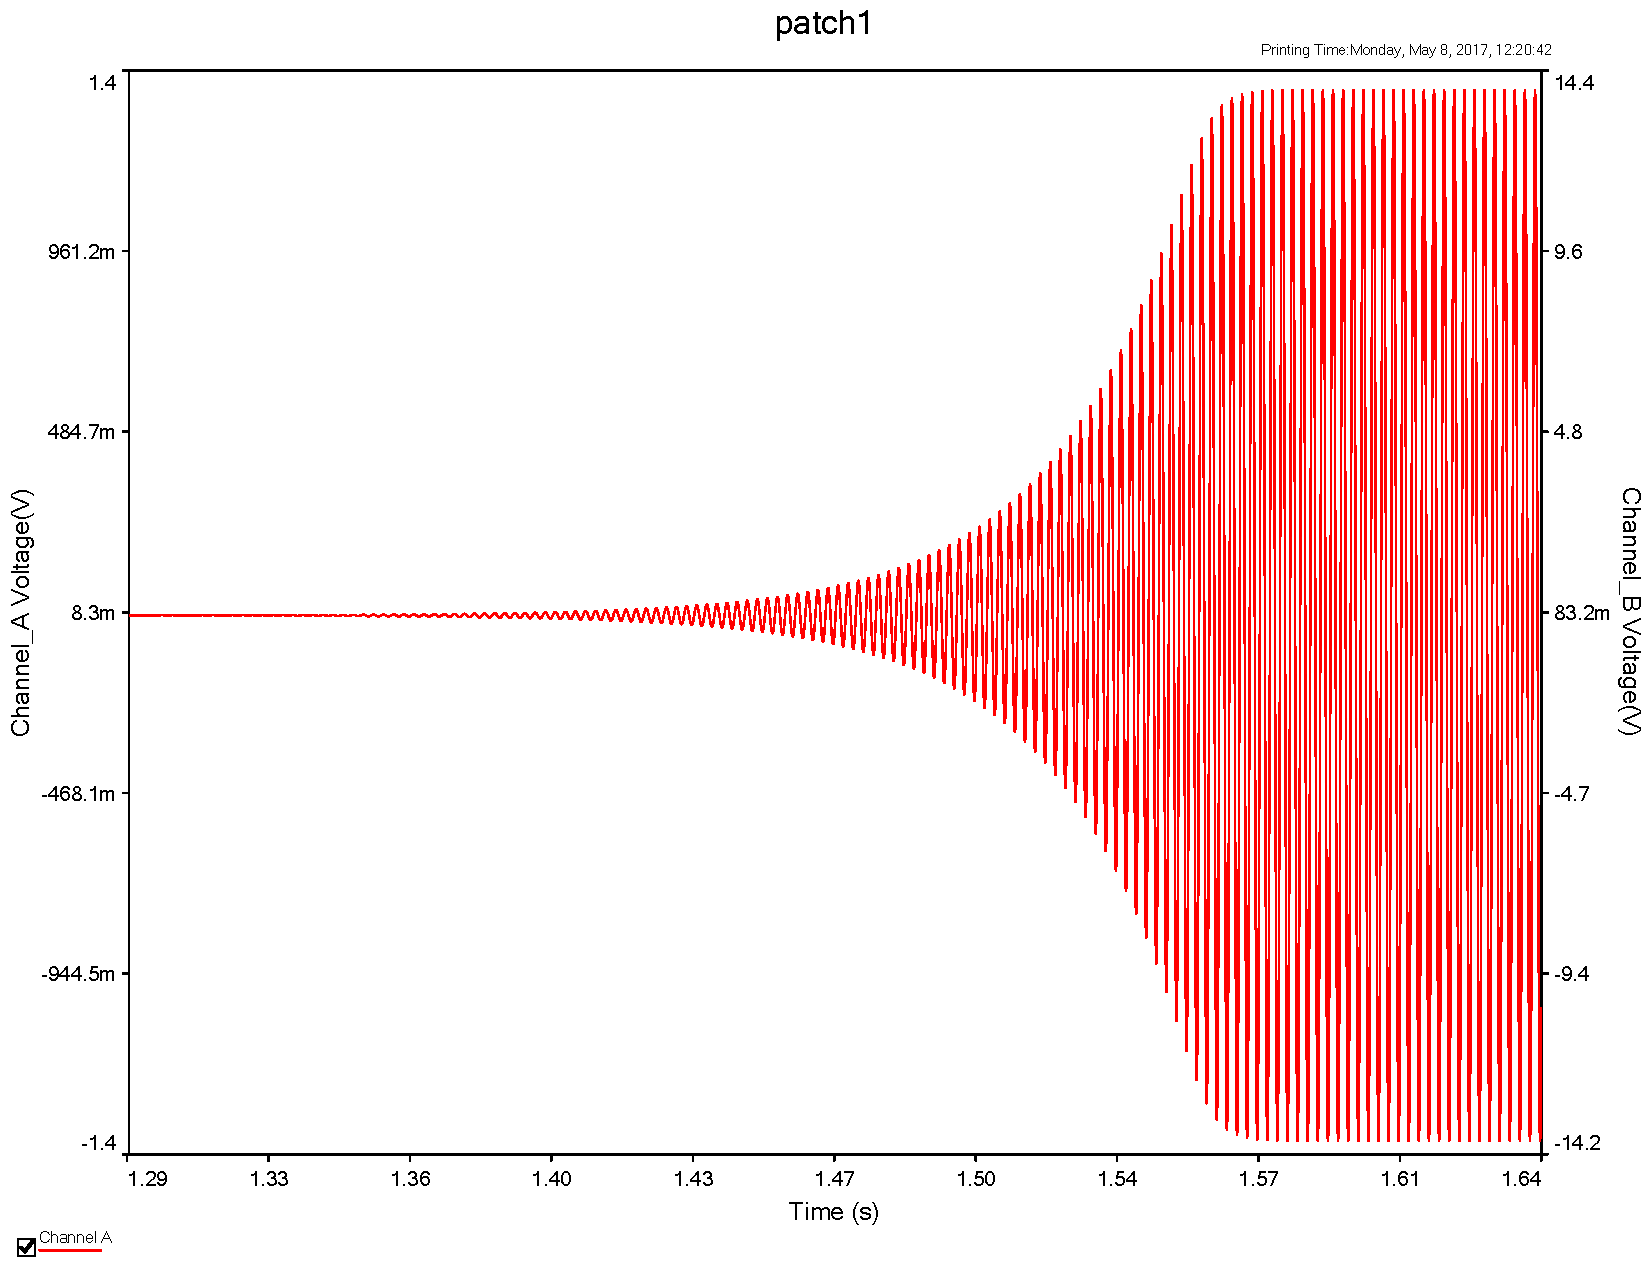
\includegraphics [width=\textwidth]{startac.pdf}
\caption{刚刚起振输出波形}
\label{ACstart}
\end {figure}
\begin{figure}[H]
\centering
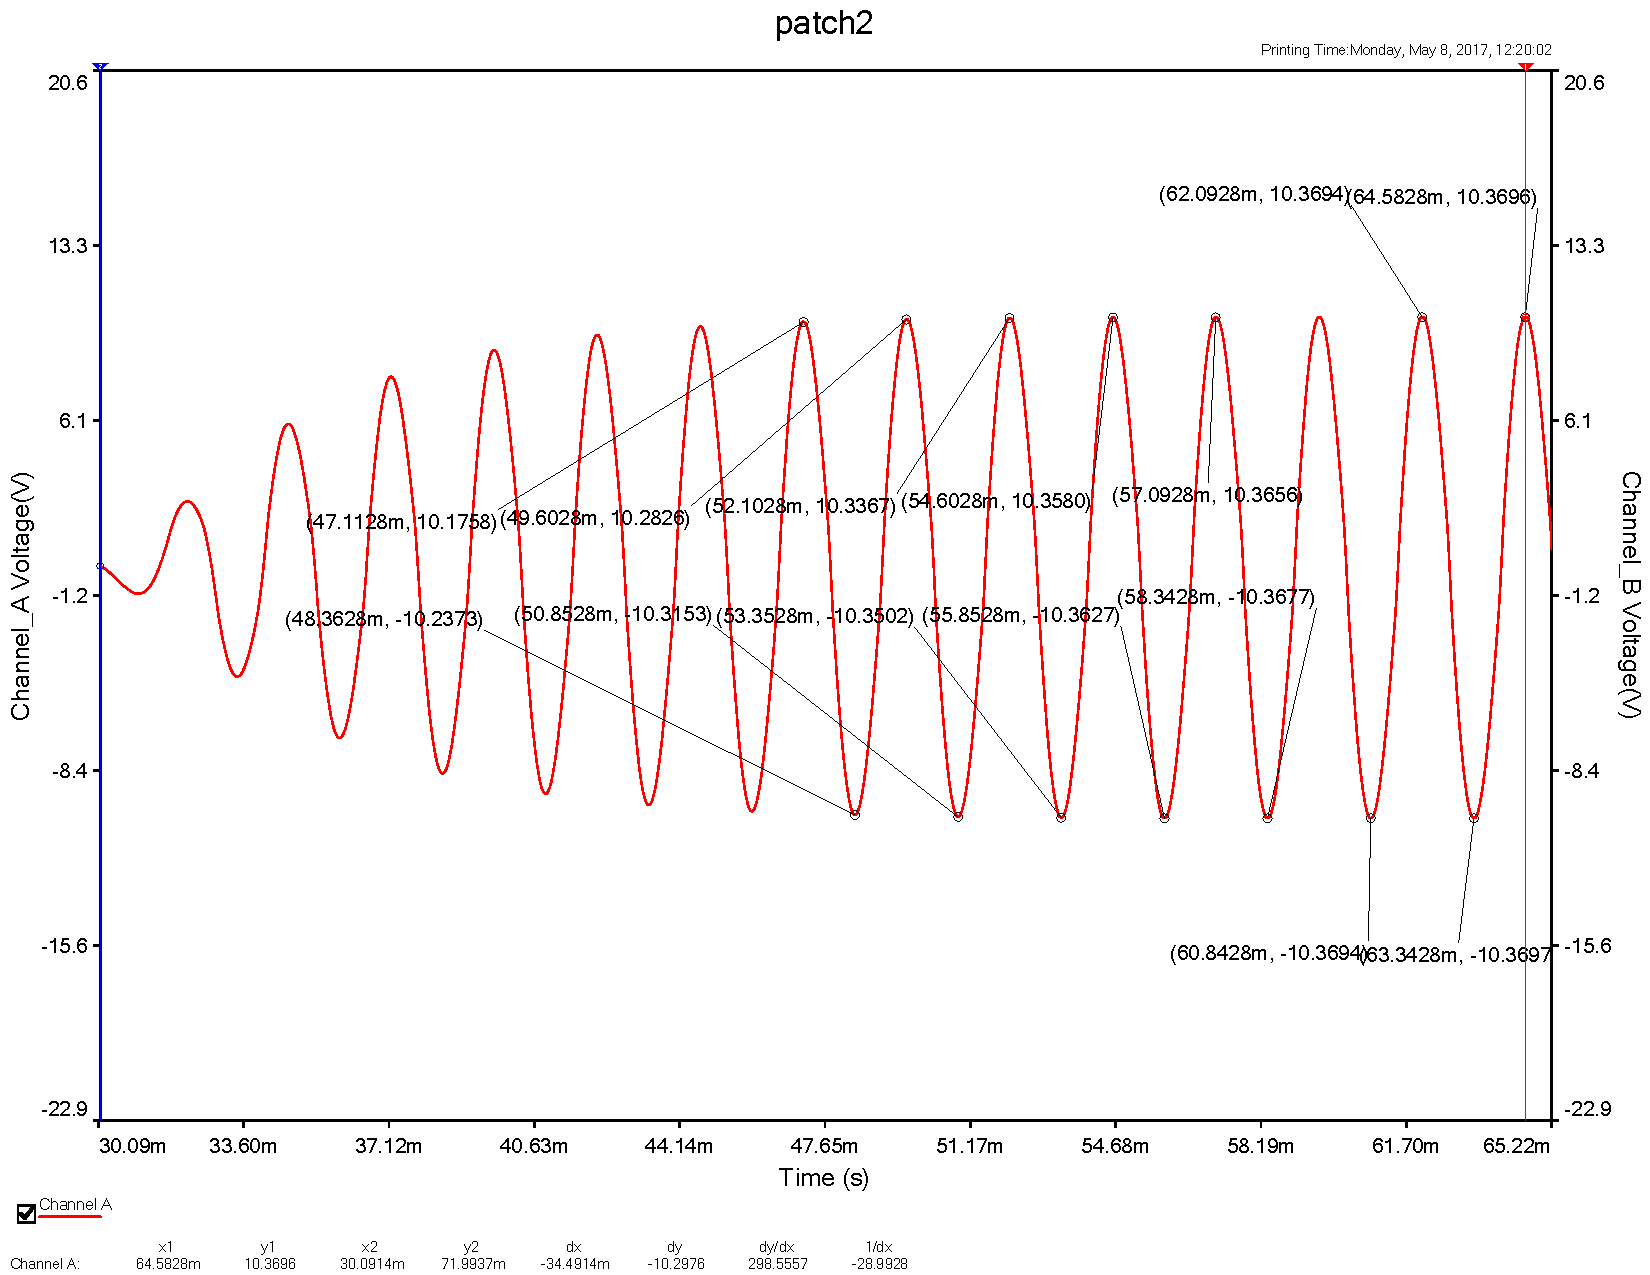
\includegraphics[width=\textwidth]{maxac.pdf}
\caption{输出最大不失真波形}
\label{ACmax}
\end{figure}
\subsubsection{其他情况的调试}
\begin{multicols}{2}
\begin{figure}[H]
\centering
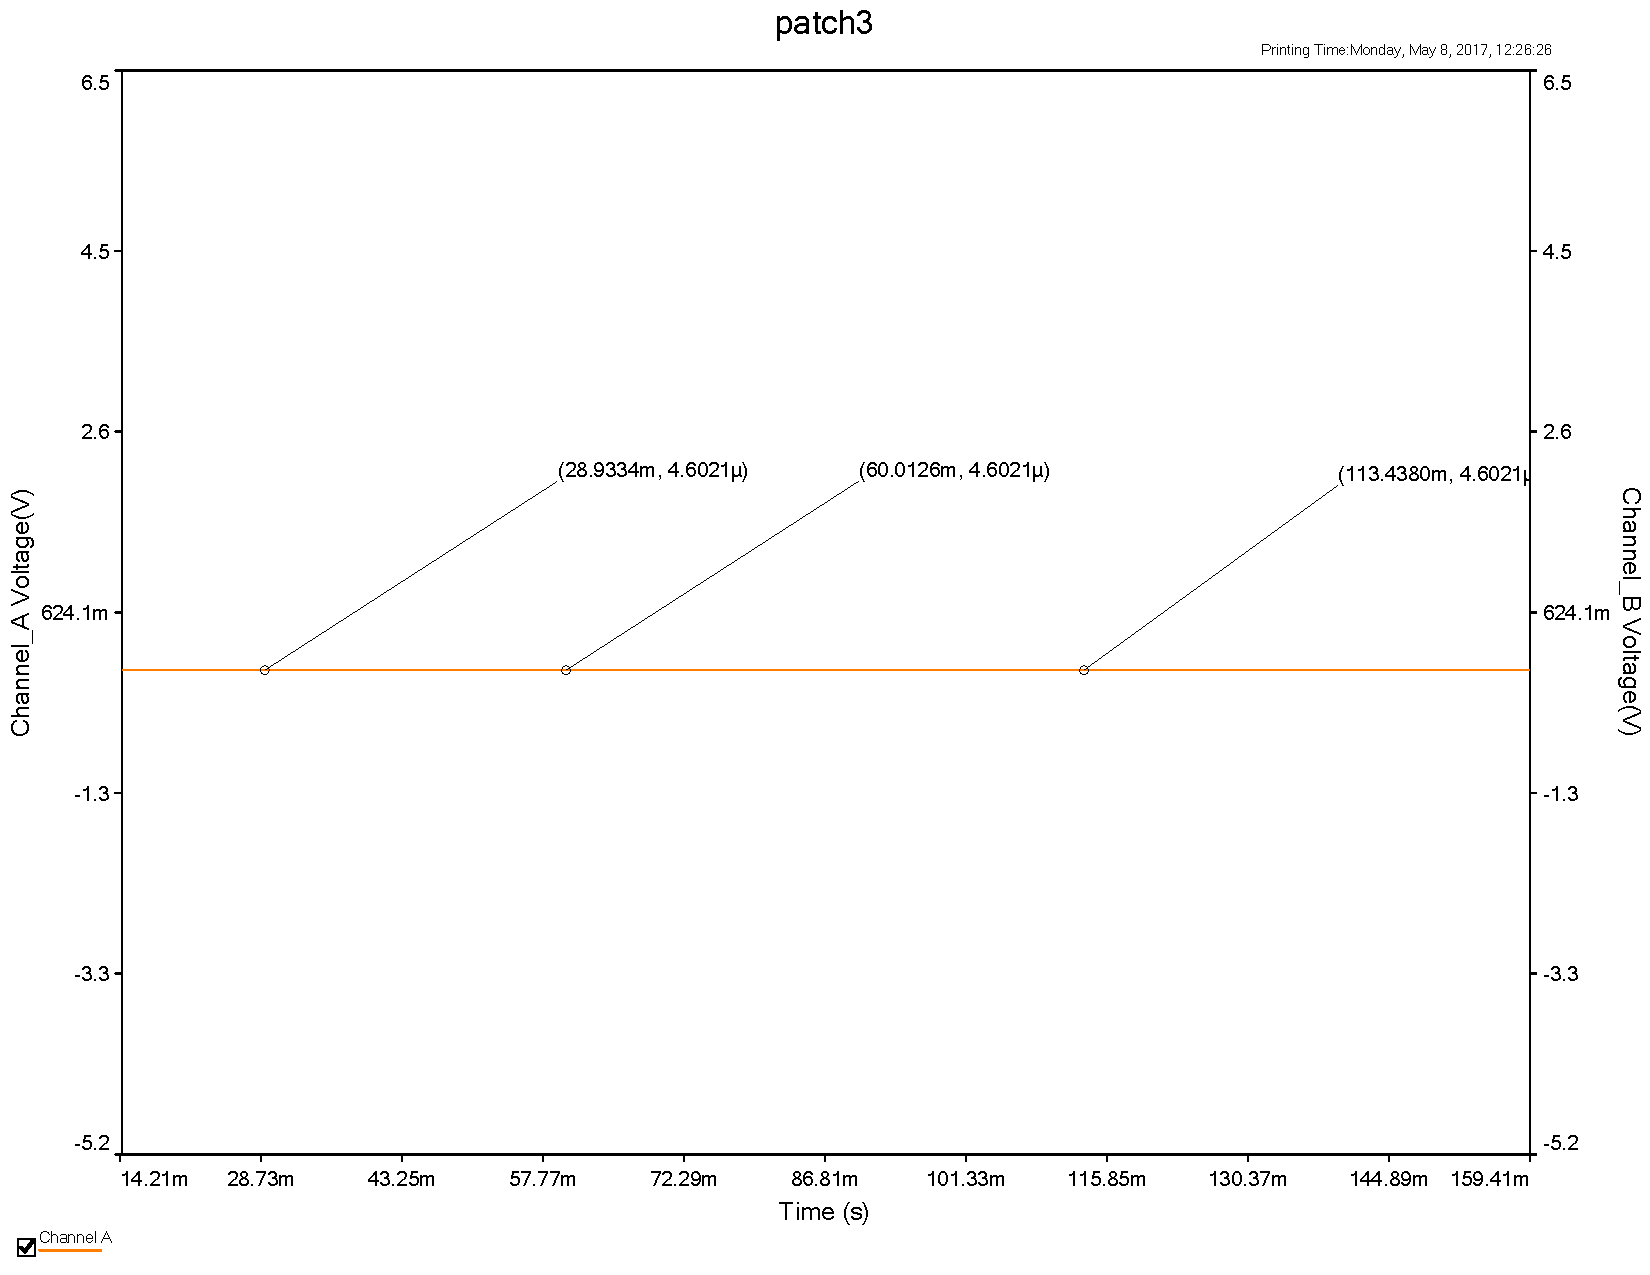
\includegraphics[width=\columnwidth]{0ac.pdf}
\caption{$R_w=20\%$时的输出波形}
\label{20}
\end{figure}
\begin{figure}[H]
\centering
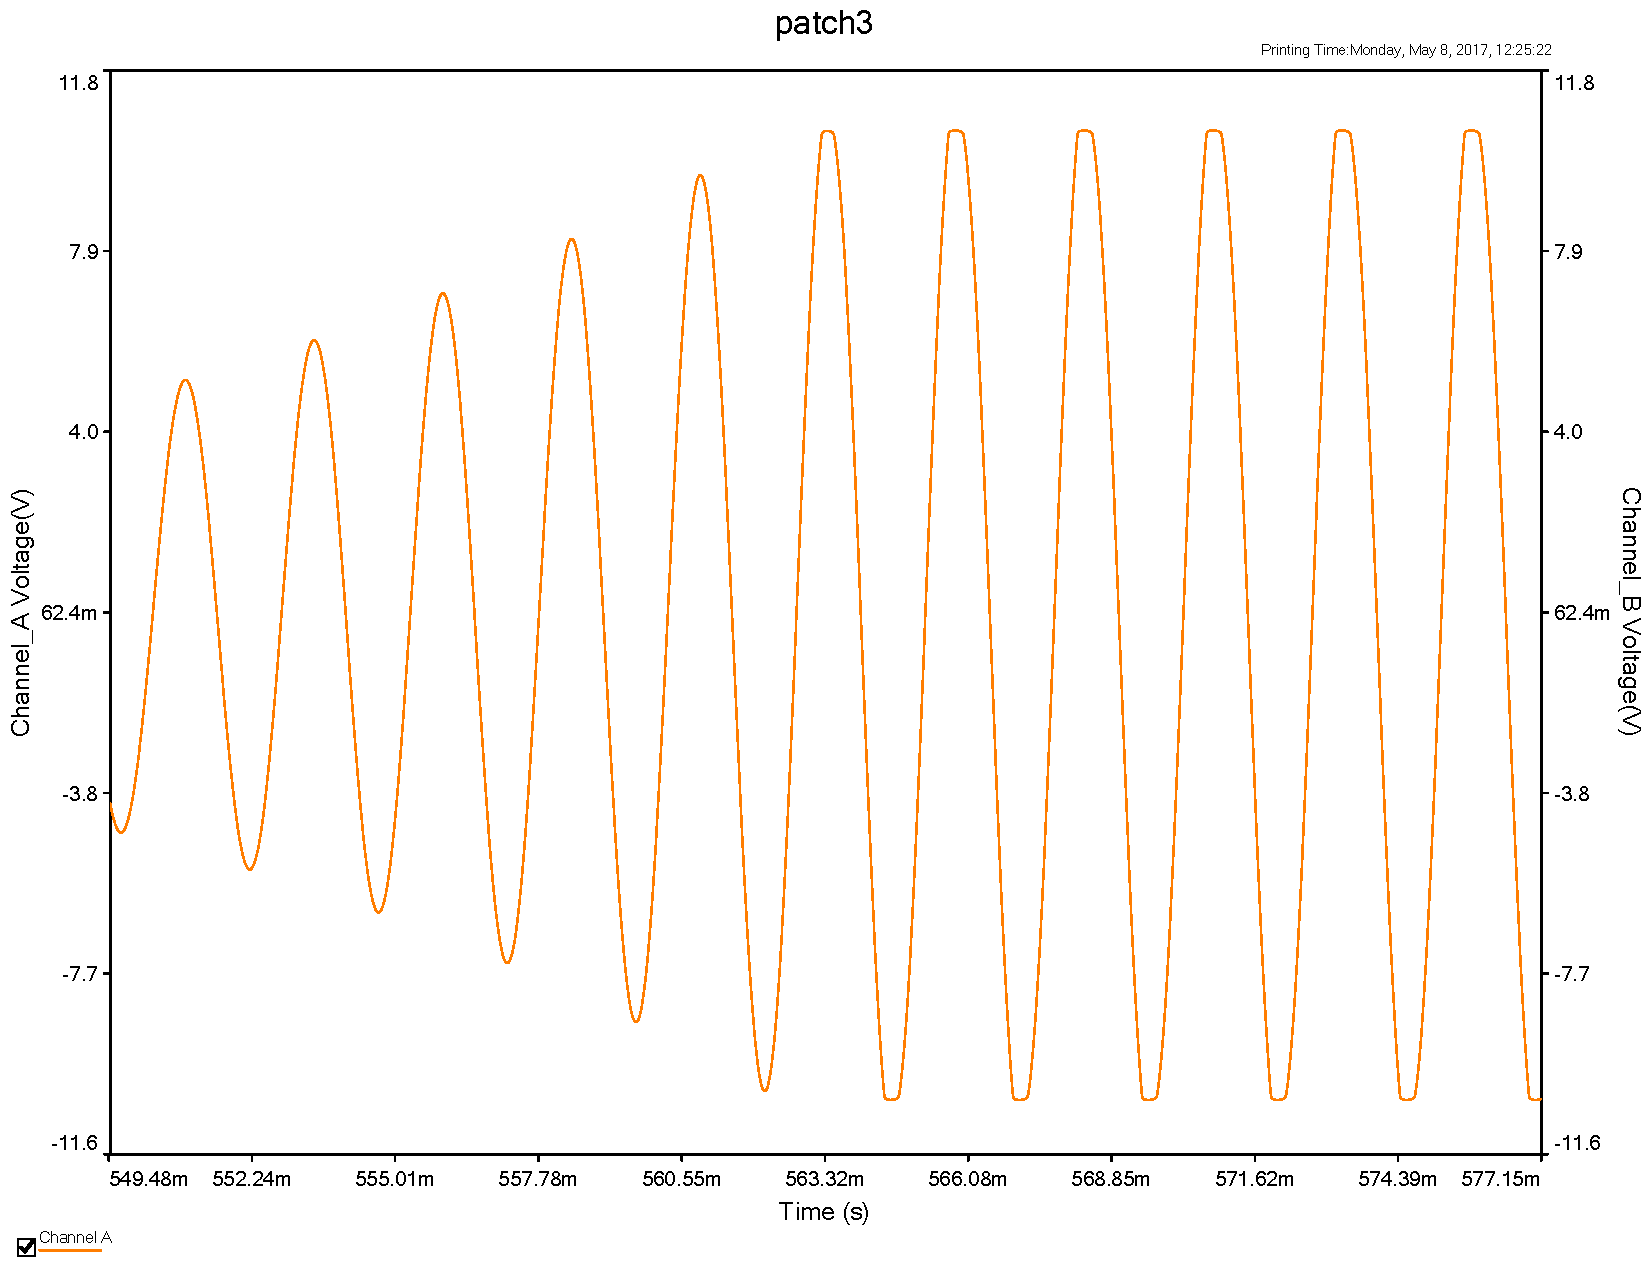
\includegraphics[width=\columnwidth]{21ac.pdf}
\caption{$R_w=21\%$时的输出波形}
\label{21}
\end{figure}
\begin{figure}[H]
\centering
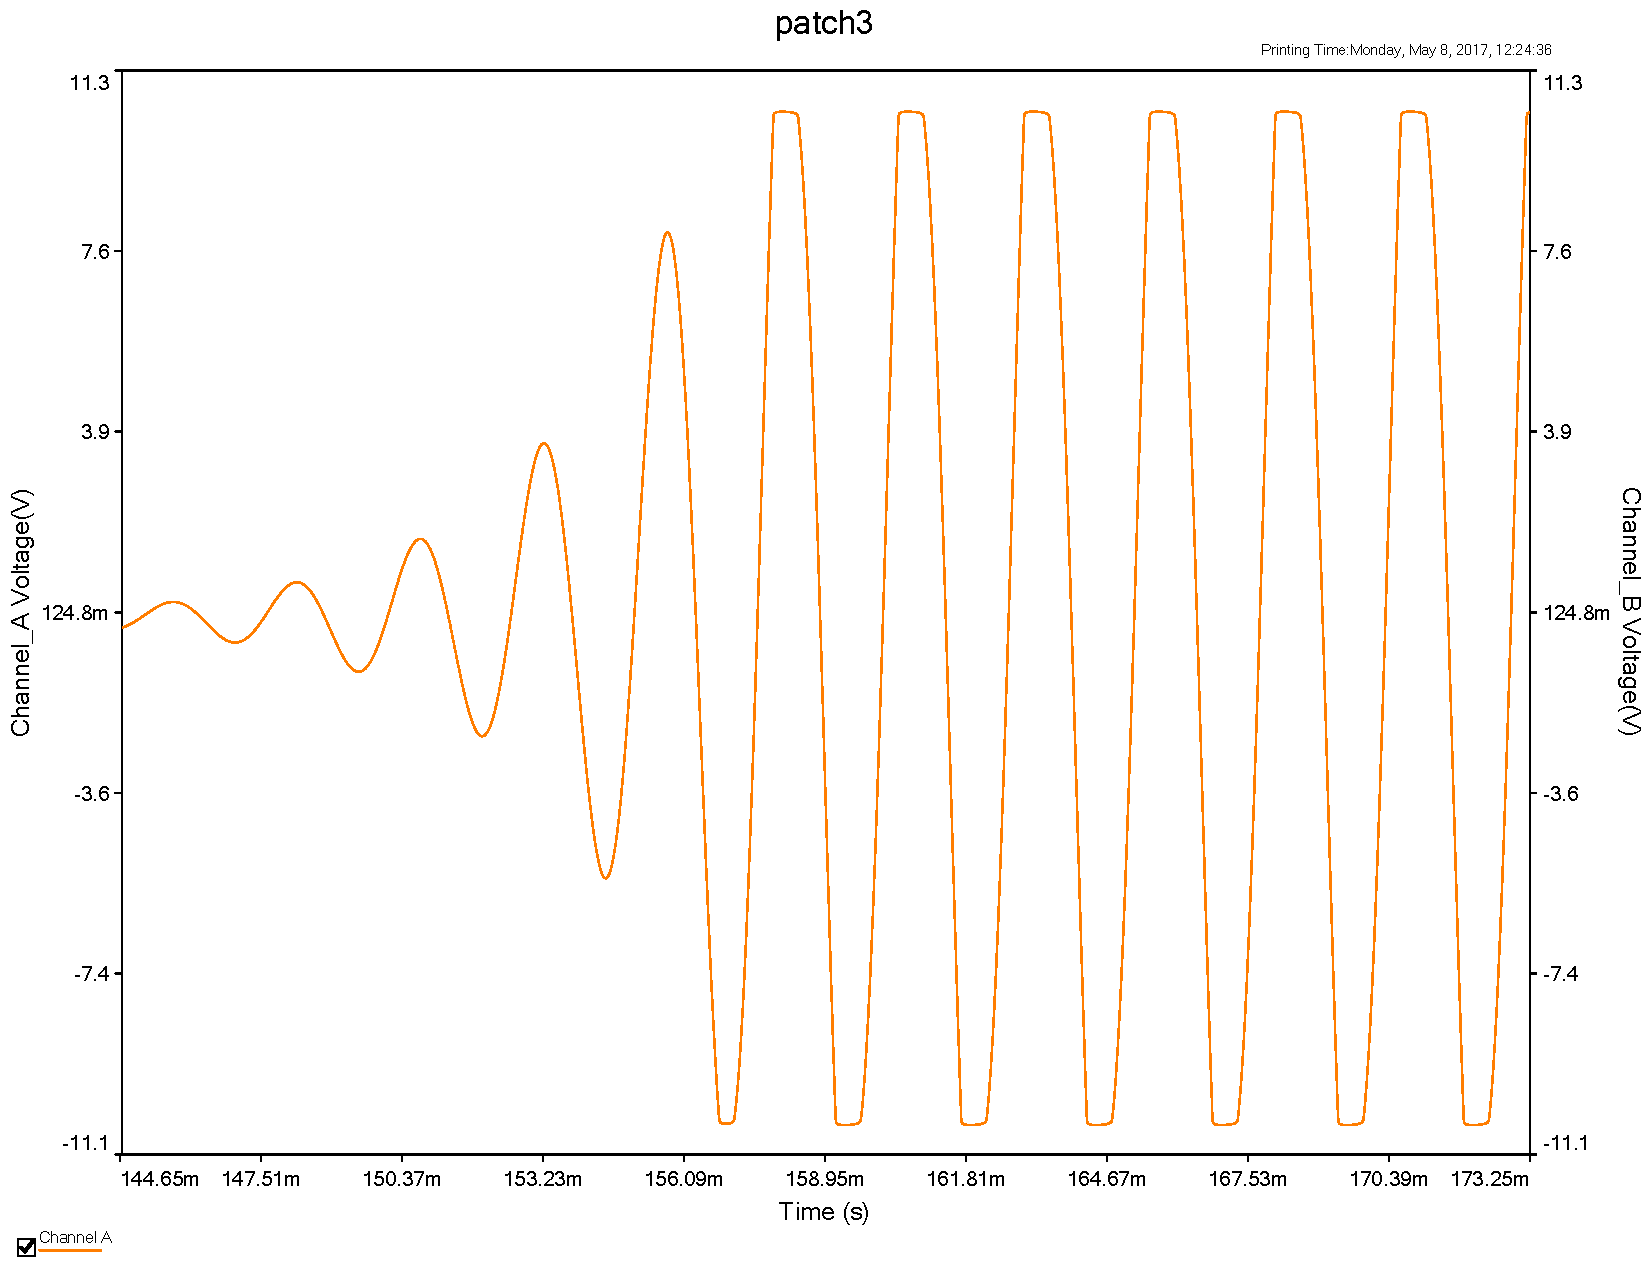
\includegraphics[width=\columnwidth]{25ac.pdf}
\caption{$R_w=25\%$时的输出波形}
\label{25}
\end{figure}
\begin{figure}[H]
\centering
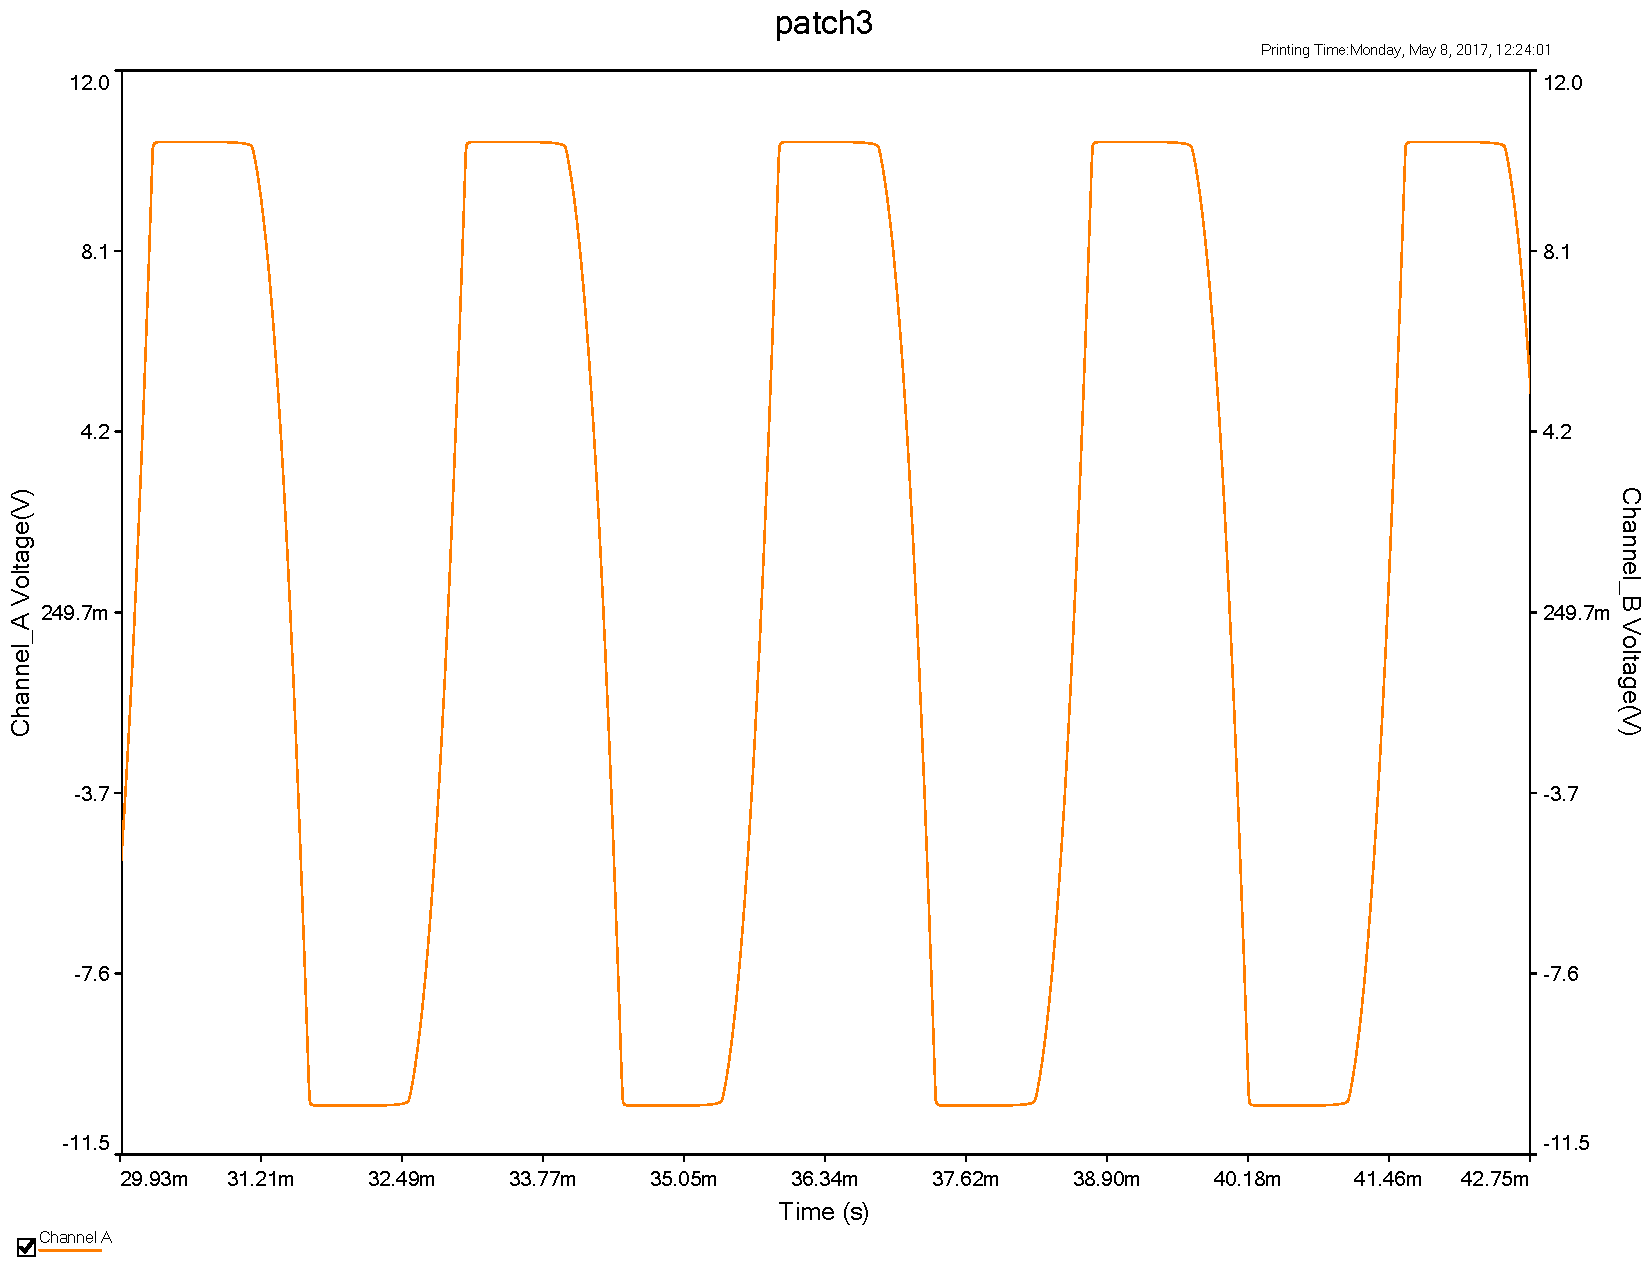
\includegraphics[width=\columnwidth]{40ac.pdf}
\caption{$R_w=40\%$时的输出波形}
\label{40}
\end{figure}
\begin{figure}[H]
\centering
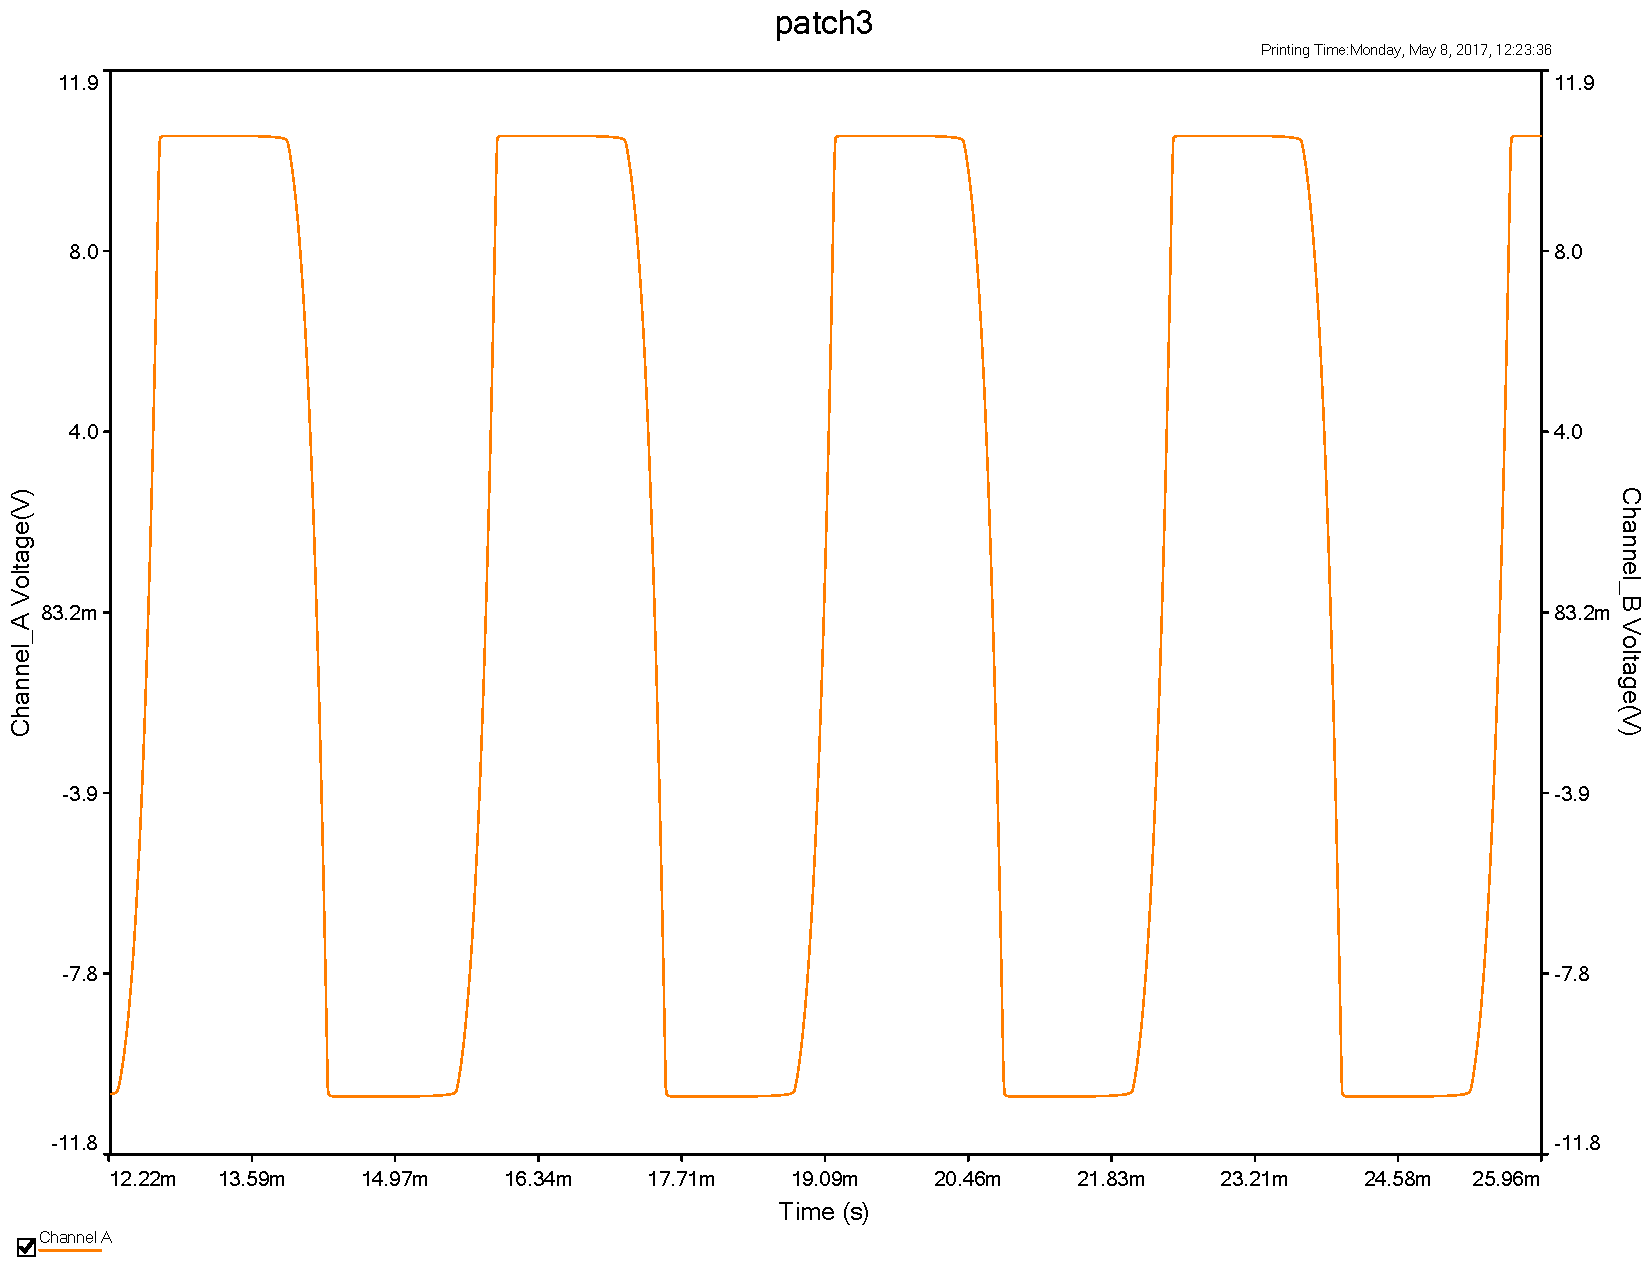
\includegraphics[width=\columnwidth]{60ac.pdf}
\caption{$R_w=60\%$时的输出波形}
\label{60}
\end{figure}
\begin{figure}[H]
\centering
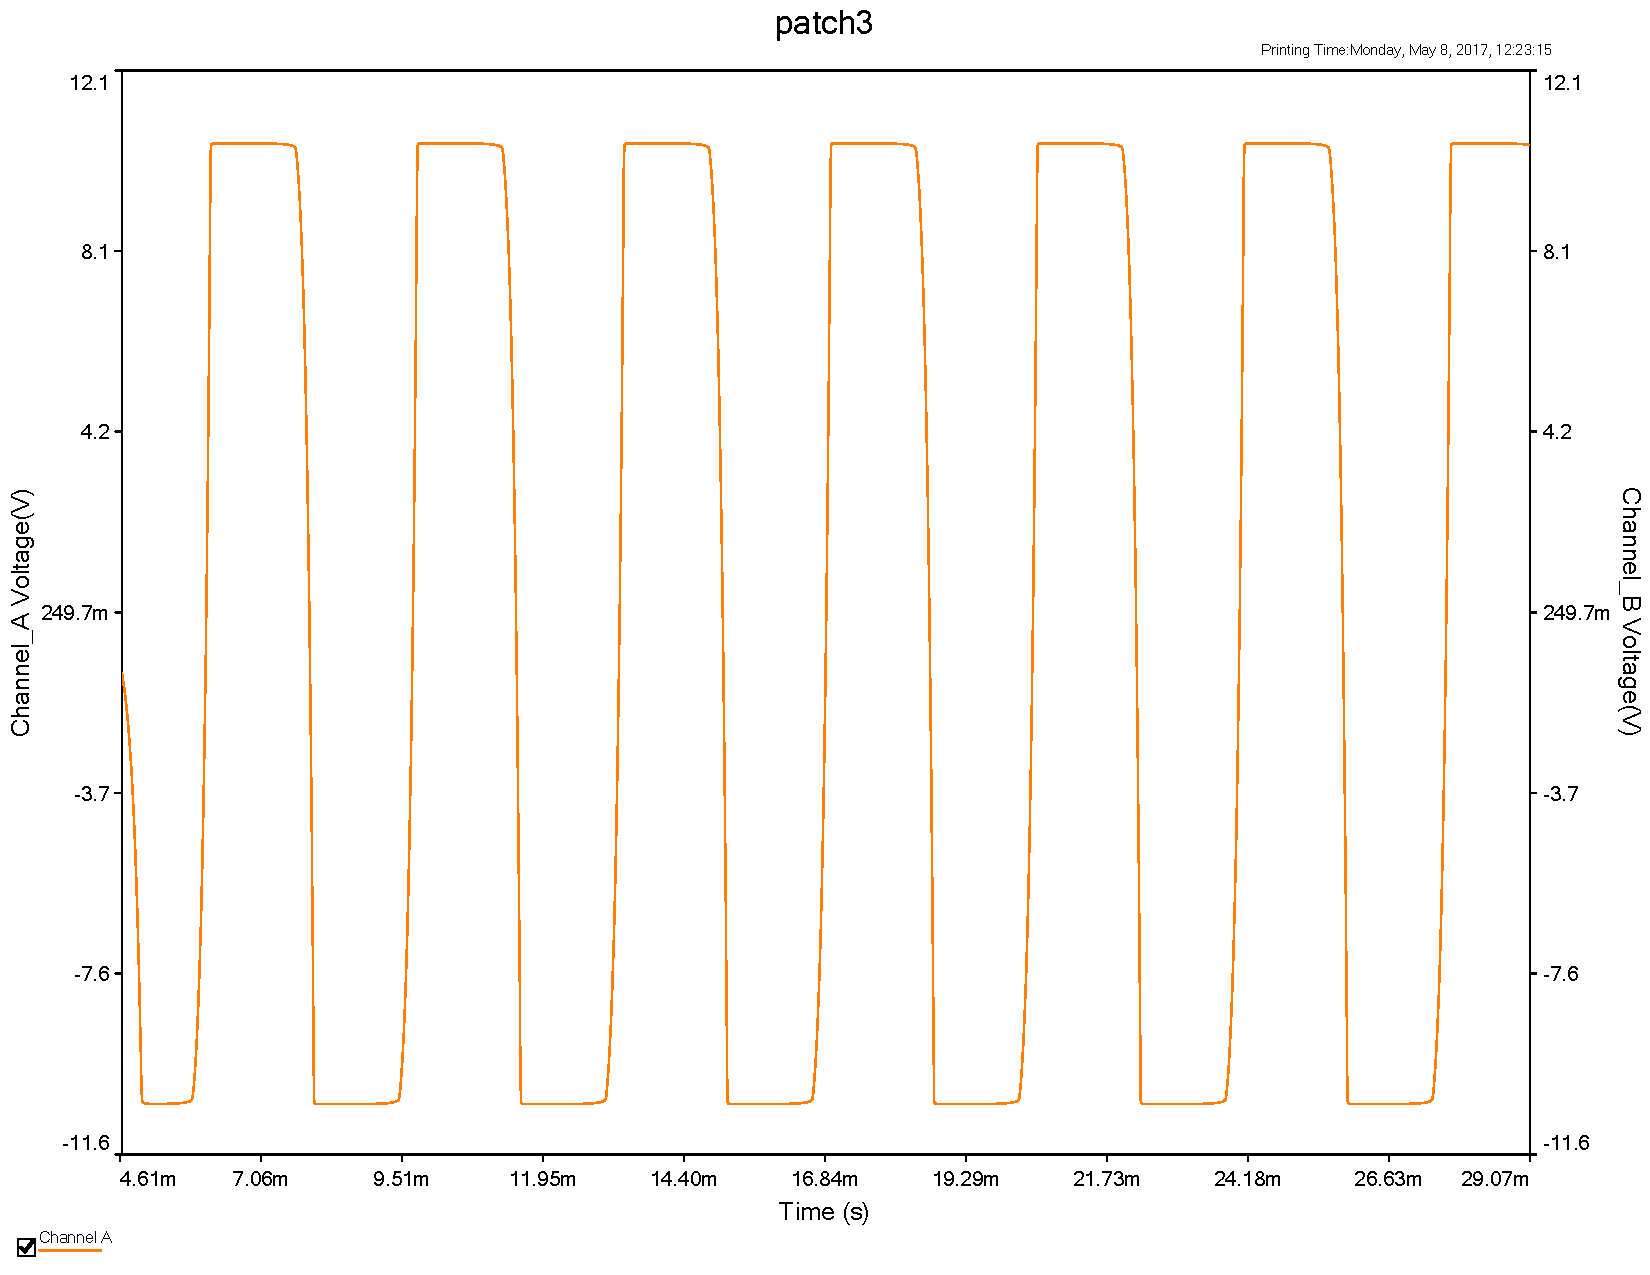
\includegraphics[width=\columnwidth]{80ac.pdf}
\caption{$R_w=80\%$时的输出波形}
\label{80}
\end{figure}
\begin{figure}[H]
\centering
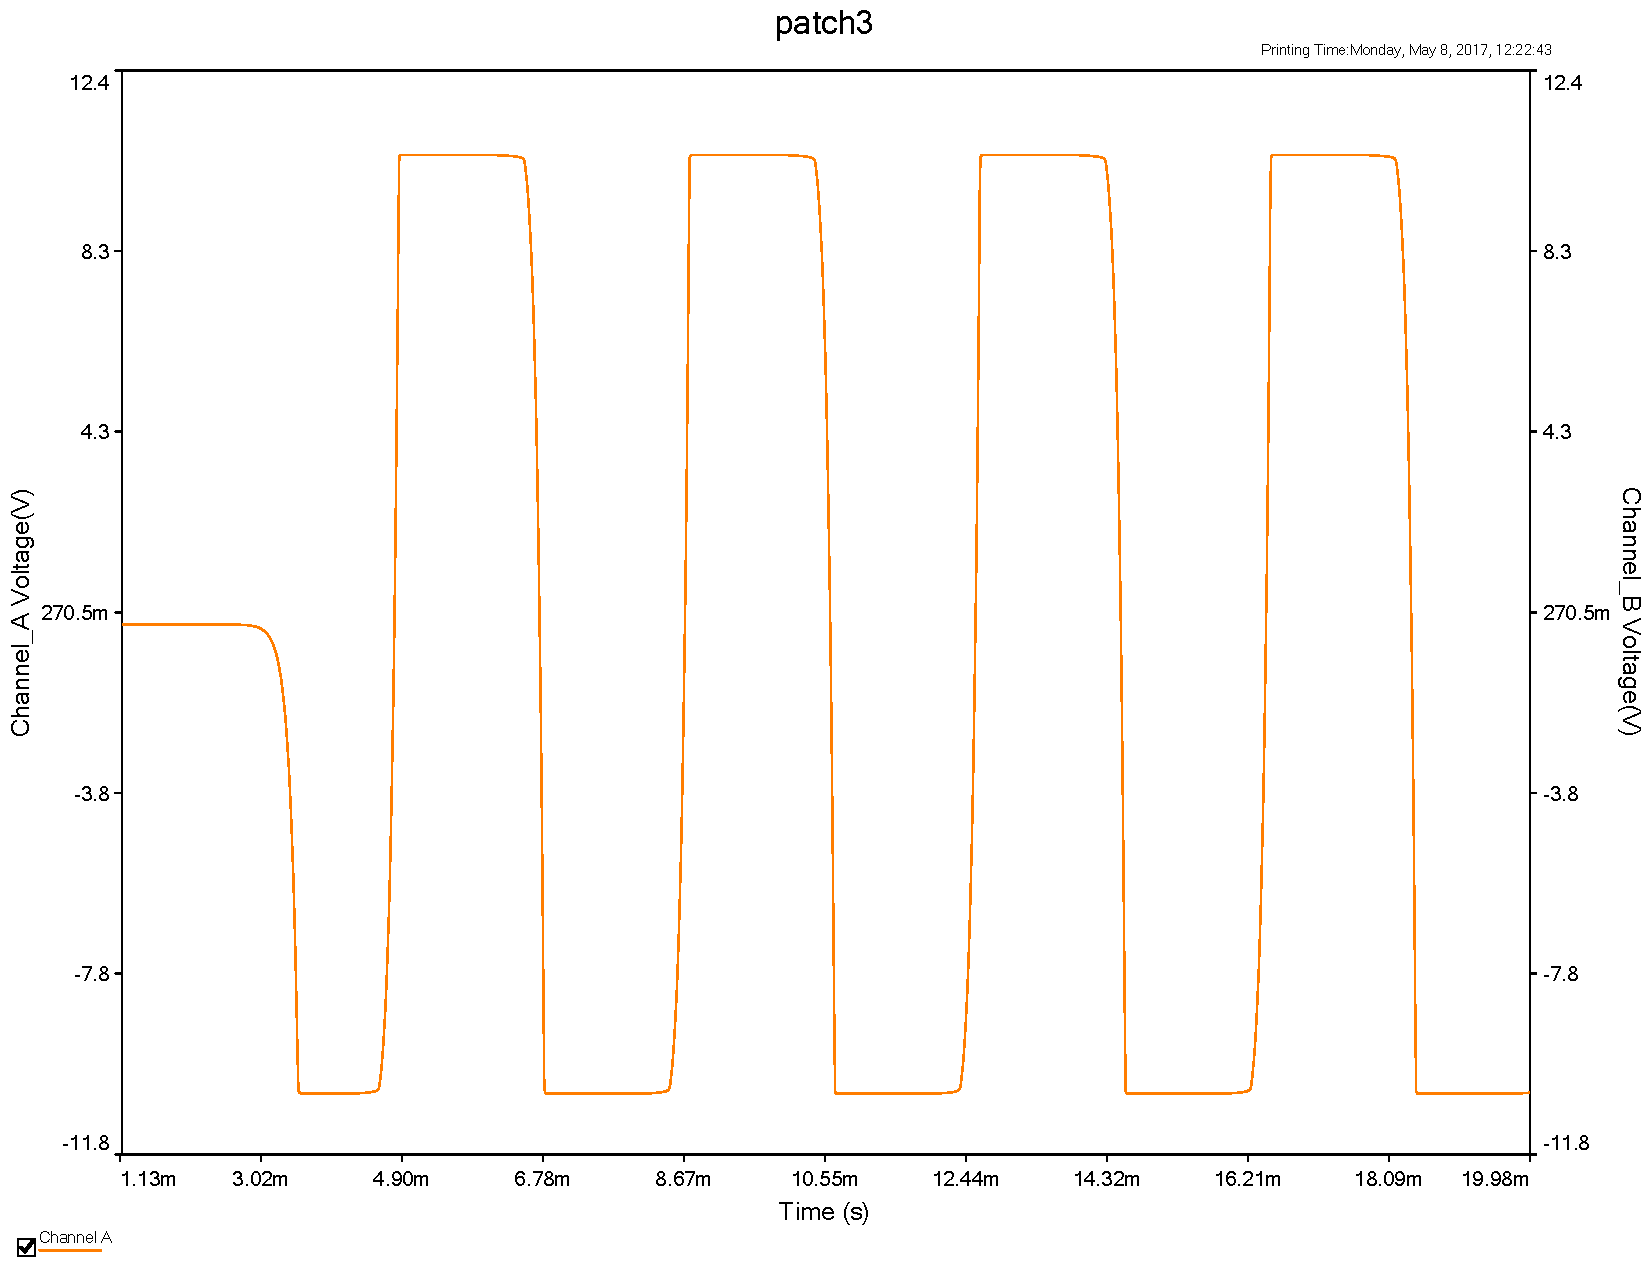
\includegraphics[width=\columnwidth]{100ac.pdf}
\caption{$R_w=100\%$时的输出波形}
\label{100}
\end{figure}
\begin{figure}[H]
\centering
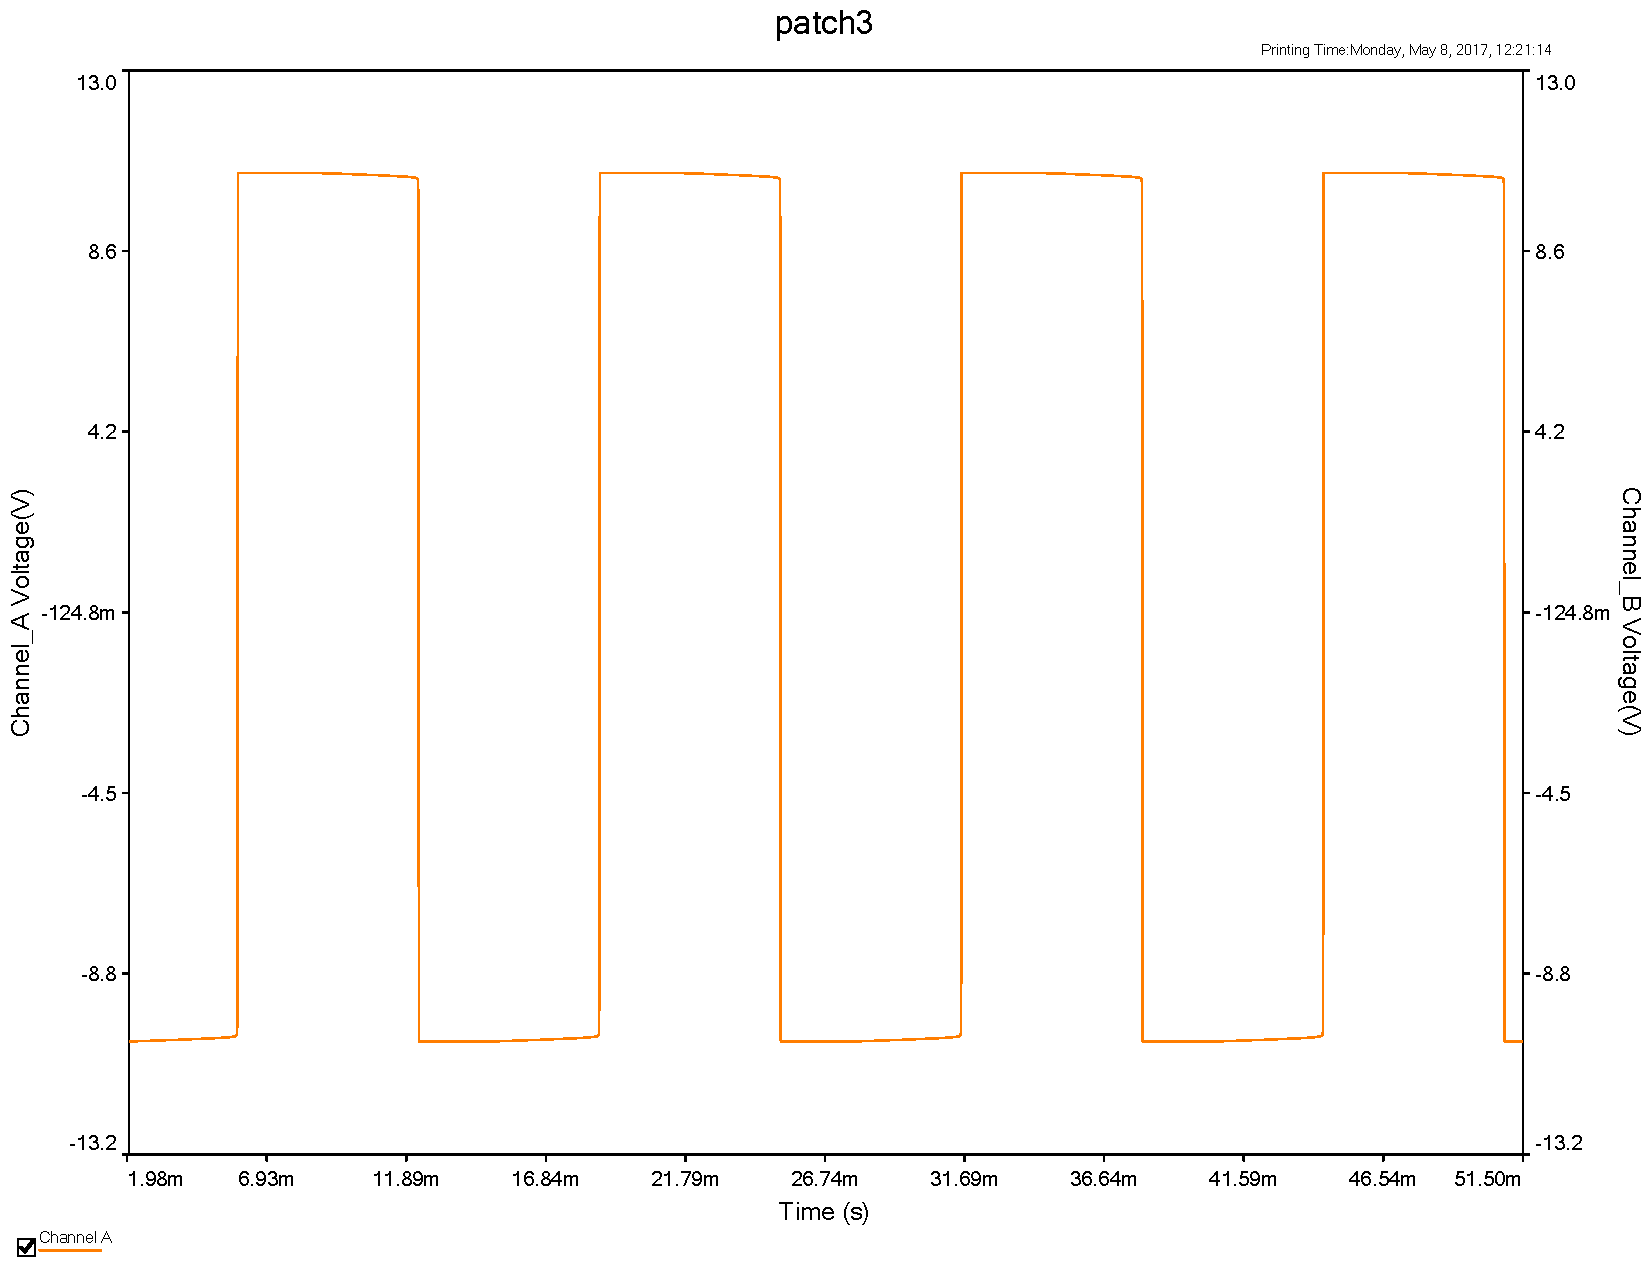
\includegraphics[width=\columnwidth]{offac.pdf}
\caption{$R_w$完全断开时的输出波形}
\label{infi}
\end{figure}
\end{multicols}
\subsection{方波——三角波发生电路}
\subsubsection{理论分析}
\begin{multicols}{2}
\begin {figure}[H]
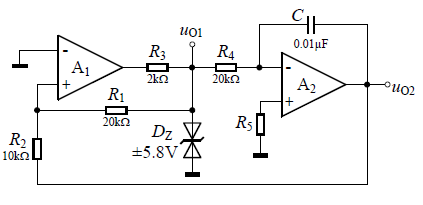
\includegraphics [width=\columnwidth]{bi.png}
\caption{方波——三角波发生电路}
\label{BICirc}
\end {figure}
\end{multicols}
\subsubsection{波形仿真}
\begin{figure}[H]
\centering
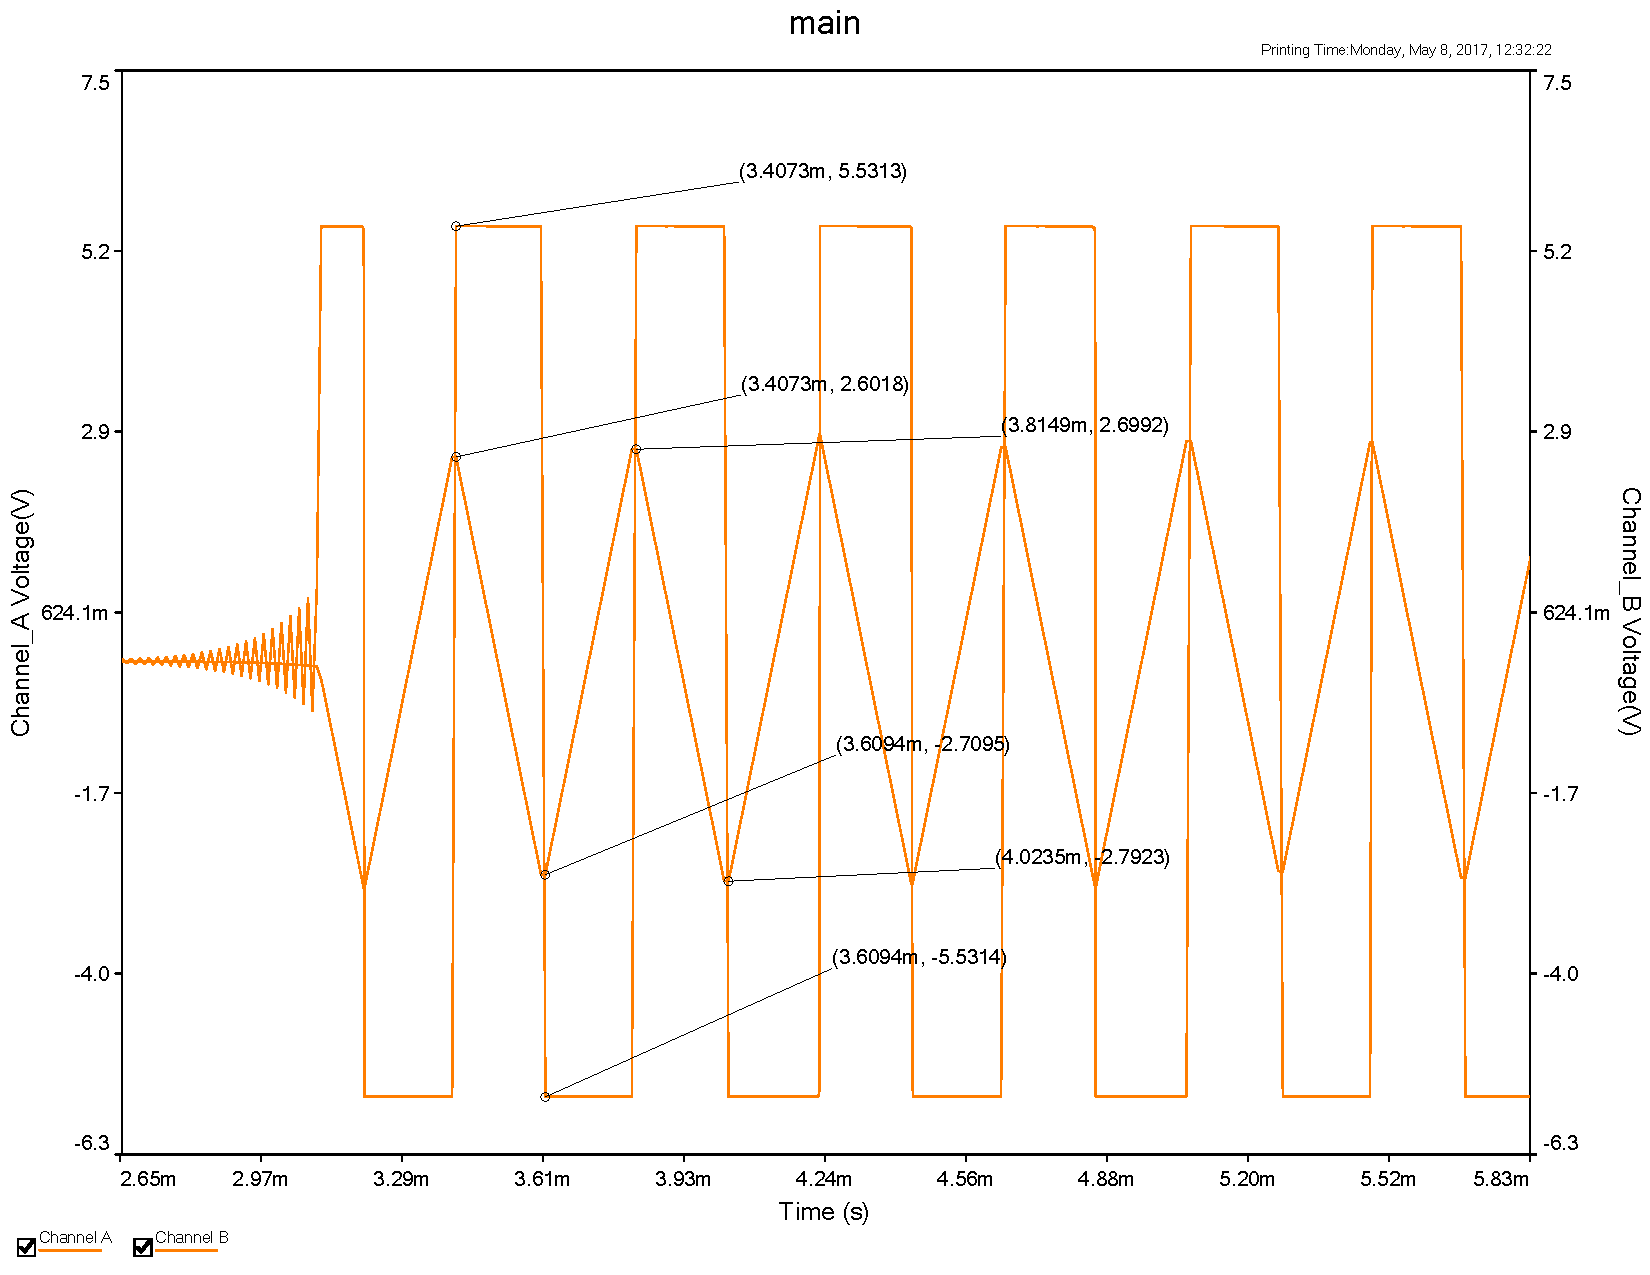
\includegraphics[width=\textwidth]{bi.pdf}
\caption{方波——三角波发生电路输出波形}
\label{BI}
\end{figure}
\subsection{滞环特性电路的测试}
\subsubsection{理论分析}
\begin {figure}[H]
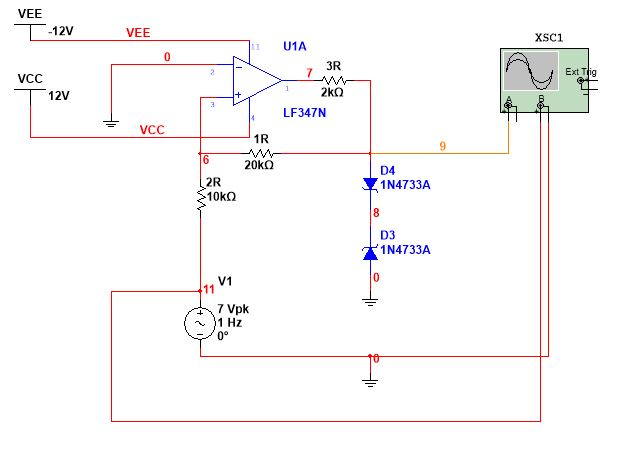
\includegraphics [width=\textwidth]{sch.jpg}
\caption{滞环特性电路}
\label{schiCrit}
\end {figure}
\subsubsection{输出波形仿真}
\begin{figure}[H]
\centering
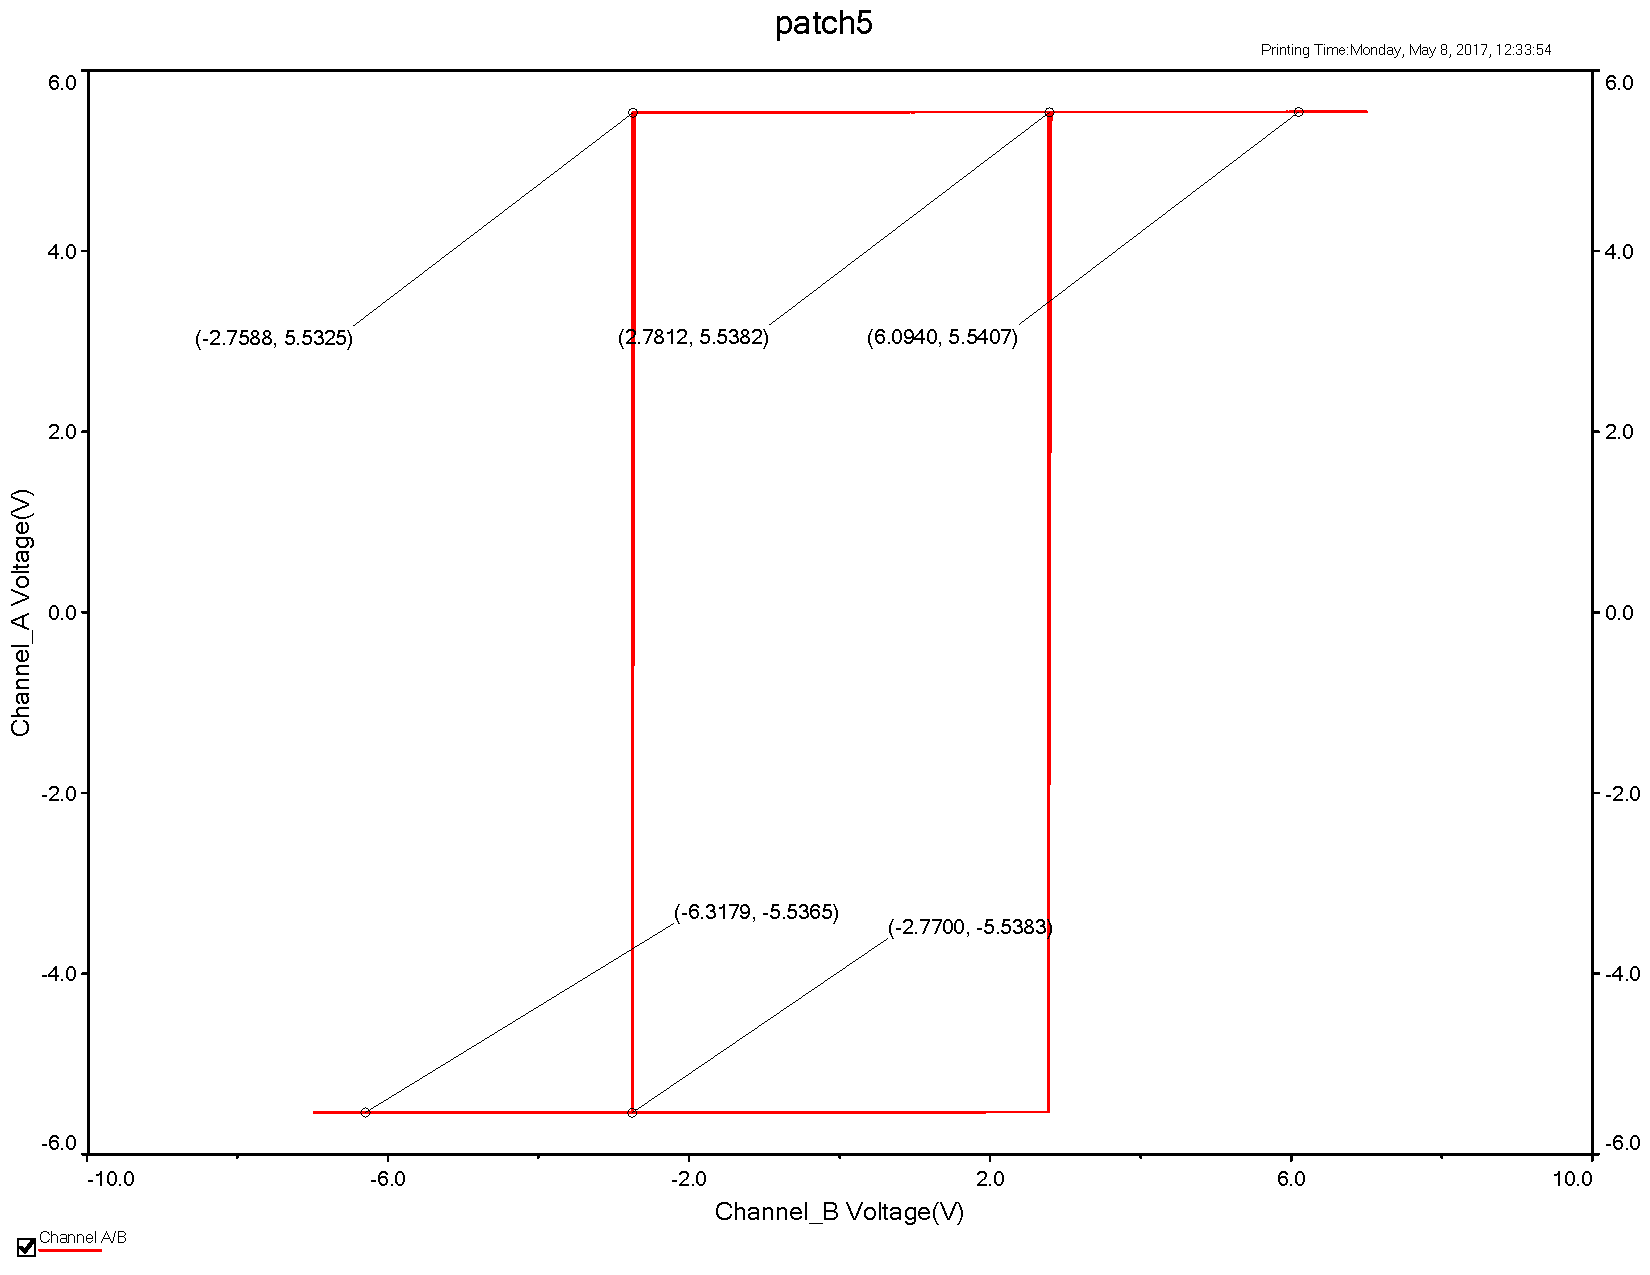
\includegraphics[width=\textwidth]{sch.pdf}
\caption{滞环特性输出波形}
\label{BI}
\end{figure}
\subsection{锯齿波发生电路}
\subsubsection{理论分析}
\begin {figure}[H]
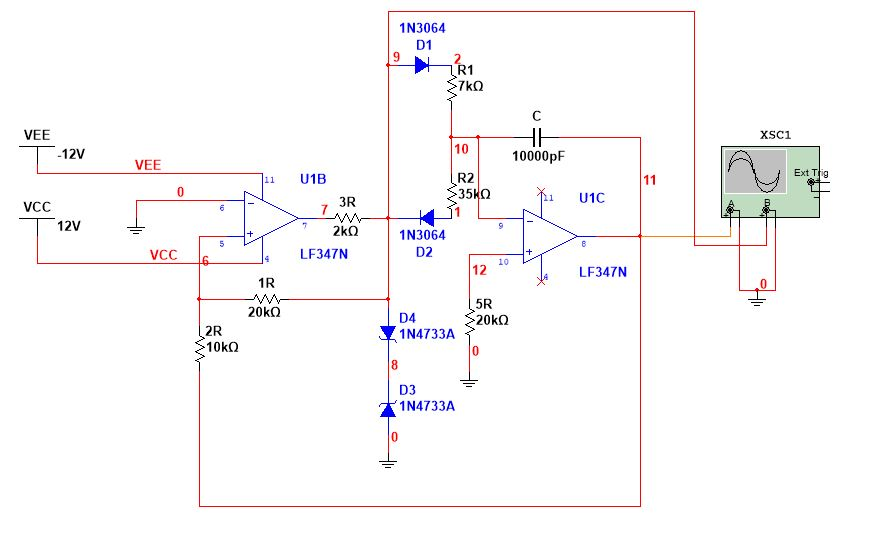
\includegraphics [width=\textwidth]{tan.jpg}
\caption{锯齿波发生电路}
\label{tanCrit}
\end {figure}
\subsubsection{输出波形仿真}
\begin{figure}[H]
\centering
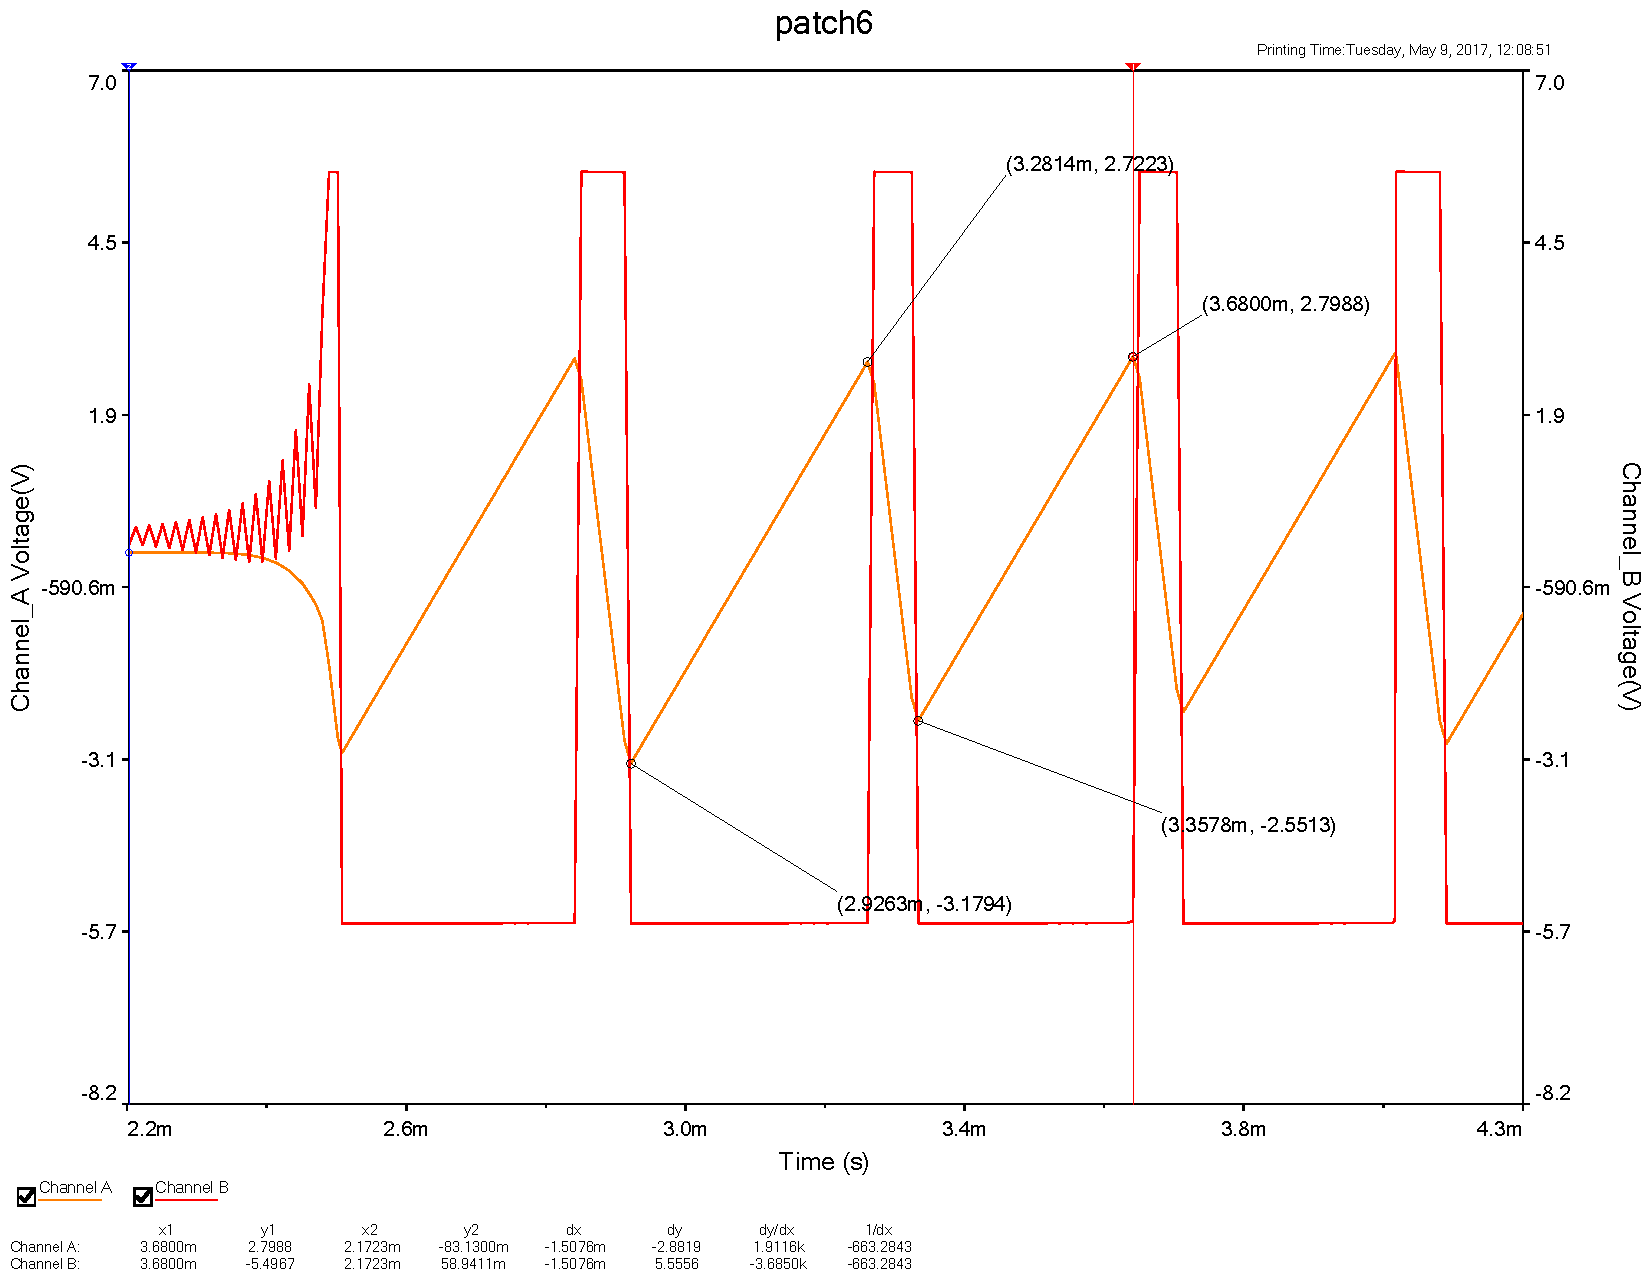
\includegraphics[width=\textwidth]{tan.pdf}
\caption{锯齿波发生电路输出波形}
\label{BI}
\end{figure}
\section{实验数据记录}
\subsection{正弦波发生电路}
\subsection{方波——三角波发生电路}
\subsection{滞环特性电路的测试}
\subsection{锯齿波发生电路}
\end{document}